% ------------------------------------------------------------------------------
% TYPO3 CMS 8.3 - What's New - Chapter "Introduction" (English Version)
%
% @author	Michael Schams <schams.net>
% @license	Creative Commons BY-NC-SA 3.0
% @link		http://typo3.org/download/release-notes/whats-new/
% @language	English
% ------------------------------------------------------------------------------
% LTXE-CHAPTER-UID:		7fdf26cc-362160ab-d6c8b905-19722b20
% LTXE-CHAPTER-NAME:	Introduction
% ------------------------------------------------------------------------------

\section{Introduzione}
\begin{frame}[fragile]
	\frametitle{Introduzione}

	\begin{center}\huge{Introduzione}\end{center}
	\begin{center}\huge{\color{typo3darkgrey}\textbf{I fatti in breve}}\end{center}

\end{frame}

% ------------------------------------------------------------------------------
% LTXE-SLIDE-START
% LTXE-SLIDE-UID:		181e6720-85864c2b-0104b839-c951c454
% LTXE-SLIDE-ORIGIN:	ca3596df-e5f14953-556d9c5f-a8a689fe English
% LTXE-SLIDE-TITLE:		TYPO3 CMS 8.2 and 8.3 - The Facts
% ------------------------------------------------------------------------------
\begin{frame}[fragile]
	\frametitle{Introduzione}
	\framesubtitle{TYPO3 CMS 8.2 e 8.3 - I fatti in breve}

	\textbf{TYPO3 CMS 8.2}
	\begin{itemize}
		\item Data di rilascio: 05 Luglio 2016
		\item Tipo di rilascio: Sprint Release
		\item Slogan: Upgrades
	\end{itemize}

	\vspace{0.6cm}

	\textbf{TYPO3 CMS 8.3}
	\begin{itemize}
		\item Data di rilascio: 30 Agosto 2016
		\item Tipo di rilascio: Sprint Release
		\item Slogan: Frontend Editing on Steroids
	\end{itemize}

%	\begin{figure}
%		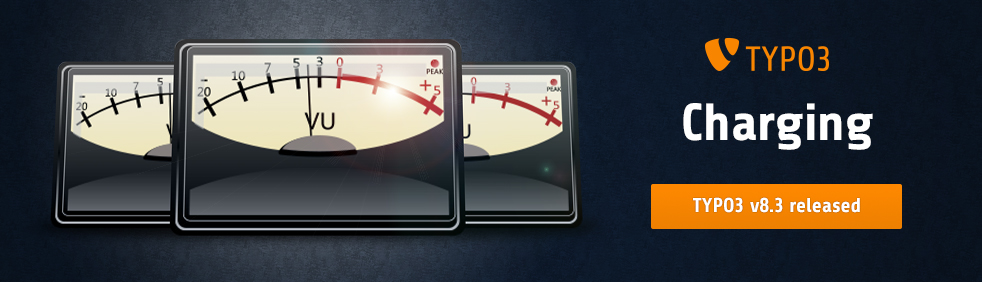
\includegraphics[width=0.95\linewidth]{Introduction/typo3cms83-banner.jpg}
%	\end{figure}

\end{frame}

% ------------------------------------------------------------------------------
% LTXE-SLIDE-START
% LTXE-SLIDE-UID:		0da54501-0efcaebb-ac4bd07e-cfa7f965
% LTXE-SLIDE-ORIGIN:	1be10378-6e990dd6-2cca609a-c778c43c English
% LTXE-SLIDE-TITLE:		System Requirements
% ------------------------------------------------------------------------------
\begin{frame}[fragile]
	\frametitle{Introduzione}
	\framesubtitle{Requisiti di sistema}

	\begin{itemize}
		\item PHP:\tabto{2.2cm}versione 7
		\item MySQL:\tabto{2.2cm}versione da 5.5 a 5.7
		\item Spazio disco:\tabto{2.2cm}min 200 MB
		\item Impostazioni PHP:

			\begin{itemize}
				\item \texttt{memory\_limit} >= 128M
				\item \texttt{max\_execution\_time} >= 240s
				\item \texttt{max\_input\_vars} >= 1500
				\item l'opzione di compilazione \texttt{-}\texttt{-disable-ipv6} \underline{non} deve essere usata
			\end{itemize}

		\item Il Backend richiede Microsoft Internet Explorer 11 o superiore,
			Microsoft Edge, Google Chrome, Firefox, Safari o altro browser recente
			e compatibile

	\end{itemize}

\end{frame}

% ------------------------------------------------------------------------------
% LTXE-SLIDE-START
% LTXE-SLIDE-UID:		1b7b0750-ffd897e9-ee94d64b-5561f811
% LTXE-SLIDE-ORIGIN:	ed8e8933-d90001c7-f7548bd3-80e549cb English
% LTXE-SLIDE-TITLE:		Development And Release Timeline
% ------------------------------------------------------------------------------
\begin{frame}[fragile]
	\frametitle{Introduzione}
	\framesubtitle{Sviluppo e tempi di rilascio}

	\begin{figure}
		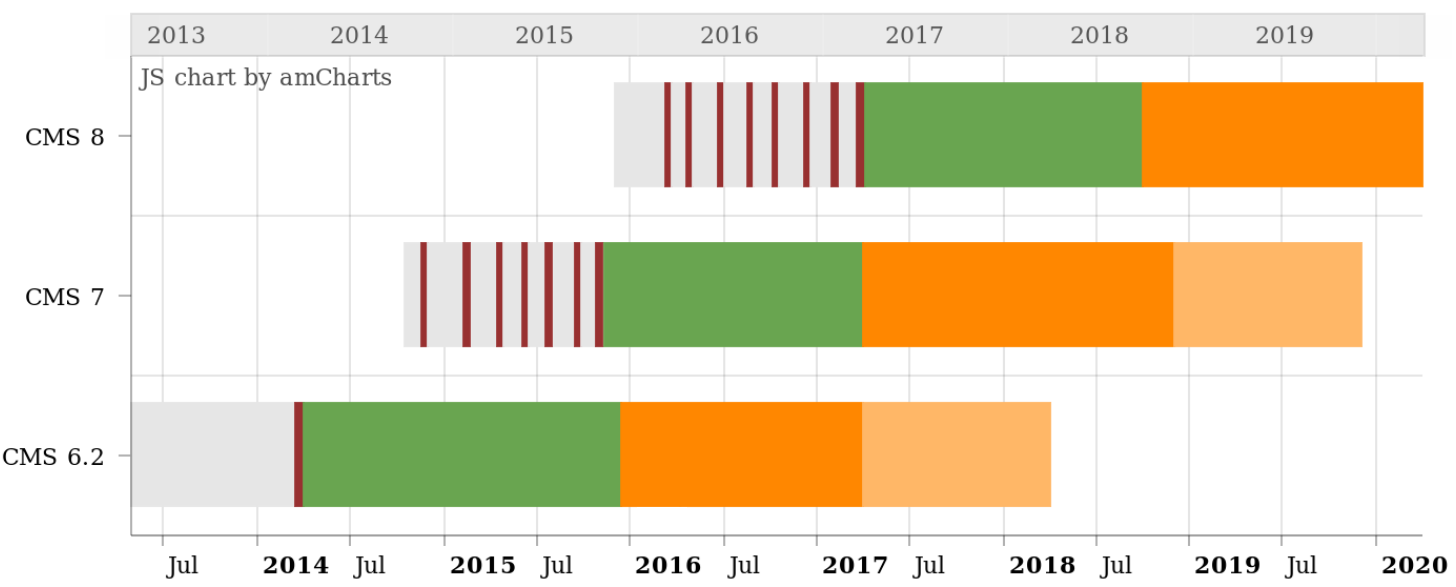
\includegraphics[width=1\linewidth]{Introduction/ReleaseAgenda.png}
	\end{figure}

\end{frame}

% ------------------------------------------------------------------------------
% LTXE-SLIDE-START
% LTXE-SLIDE-UID:		20f57eeb-af95c0a7-e6b03869-f0e9376d
% LTXE-SLIDE-ORIGIN:	01225efb-e9fdbaff-726e5fed-5b7f0003 English
% LTXE-SLIDE-TITLE:		TYPO3 CMS Roadmap
% ------------------------------------------------------------------------------
\begin{frame}[fragile]
	\frametitle{Introduzione}
	\framesubtitle{TYPO3 CMS Roadmap}

	Date di rilascio stimate e loro obiettivo principale:

	\begin{itemize}

		\item v8.0 \tabto{1.1cm}22/Mar/2016\tabto{3.4cm}Aggiunta di parti dell'ultimo momento
		\item v8.1 \tabto{1.1cm}03/Mag/2016\tabto{3.4cm}Integrazione cloud
		\item
			\begingroup
				\color{typo3orange}
					v8.2 \tabto{1.1cm}05/Lug/2016\tabto{3.4cm}Aggiornamenti
			\endgroup
		\item
			\begingroup
				\color{typo3orange}
					v8.3 \tabto{1.1cm}30/Ago/2016\tabto{3.4cm}Miglioramento dell'Editing da Frontend
			\endgroup
		\item v8.4 \tabto{1.1cm}18/Ott/2016\tabto{3.4cm}\textit{da determinare}
		\item v8.5 \tabto{1.1cm}20/Dic/2016\tabto{3.4cm}Supporto Integrazione
		\item v8.6 \tabto{1.1cm}14/Feb/2017\tabto{3.4cm}\textit{da determinare}
		\item v8.7 \tabto{1.1cm}04/Apr/2017\tabto{3.4cm}Preparazione LTS

	\end{itemize}

	\smaller
		\url{https://typo3.org/typo3-cms/roadmap/}\newline
		\url{https://typo3.org/news/article/kicking-off-typo3-v8-development/}
	\normalsize

\end{frame}

% ------------------------------------------------------------------------------
% LTXE-SLIDE-START
% LTXE-SLIDE-UID:		68e48c13-b45c3992-24e15b3d-b9238506
% LTXE-SLIDE-ORIGIN:	793cc944-52bccf17-ba7c4c9c-661e8993 English
% LTXE-SLIDE-TITLE:		Installation
% ------------------------------------------------------------------------------
\begin{frame}[fragile]
	\frametitle{Introduzione}
	\framesubtitle{Installazione}

	\begin{itemize}
		\item Procedura ufficiale di installazione su Linux/Mac OS X\newline
			(Directory Root ad esempio \texttt{/var/www/site/htdocs}):
		\begin{lstlisting}
			$ cd /var/www/site
			$ wget --content-disposition get.typo3.org/8.1
			$ tar xzf typo3_src-8.1.0.tar.gz
			$ cd htdocs
			$ ln -s ../typo3_src-8.1.0 typo3_src
			$ ln -s typo3_src/index.php
			$ ln -s typo3_src/typo3
			$ touch FIRST_INSTALL
		\end{lstlisting}

		\item Link simbolici in Microsoft Windows:

			\begin{itemize}
				\item Usa \texttt{junction} in Windows XP/2000
				\item Usa \texttt{mklink} in Windows Vista e Windows 7
			\end{itemize}

	\end{itemize}
\end{frame}

% ------------------------------------------------------------------------------
% LTXE-SLIDE-START
% LTXE-SLIDE-UID:		975c1951-56c794de-77883feb-854e178f
% LTXE-SLIDE-ORIGIN:	4c0c3586-154241f9-4c859652-03bcc92e English
% LTXE-SLIDE-TITLE:		Upgrade to TYPO3 CMS 7
% ------------------------------------------------------------------------------
\begin{frame}[fragile]
	\frametitle{Introduzione}
	\framesubtitle{Aggiornamento a TYPO3 CMS 8.x}

	\begin{itemize}
		\item Aggiornamenti possibili solo da TYPO3 CMS 7.6 LTS
		\item TYPO3 CMS < 7.6 LTS deve essere prima aggiornato a TYPO3 CMS 7.6 LTS
	\end{itemize}

	\begin{itemize}

		\item Istruzioni per l'aggiornamento:\newline
			\smaller\url{http://wiki.typo3.org/Upgrade#Upgrading_to_8.3}\normalsize
		\item Guida ufficiale TYPO3 "TYPO3 Installation and Upgrading":
			\smaller\url{http://docs.typo3.org/typo3cms/InstallationGuide}\normalsize
		\item Approcio generale:
			\begin{itemize}
				\item Verifica i requisiti minimi di sistema \small(PHP, MySQL, etc.)
				\item Verifica \textbf{deprecation\_*.log} nella vecchia istanza TYPO3
				\item Aggiorna tutte le estensioni all'ultima versione
				\item Imposta il nuovo sorgente ed esegui Install Tool -> Upgrade Wizard
				\item Verifica il modulo di startup per gli utenti di backend (opzionale)
			\end{itemize}
	\end{itemize}

\end{frame}

% ------------------------------------------------------------------------------

% ------------------------------------------------------------------------------
% LTXE-SLIDE-START
% LTXE-SLIDE-UID:		50440d8c-ff613455-2f5177ba-4f977c04
% LTXE-SLIDE-ORIGIN:	36c478bf-991c3c9c-1b55ed59-ee1ad72e English
% LTXE-SLIDE-TITLE:		PHP Version 7
% ------------------------------------------------------------------------------
\begin{frame}[fragile]
	\frametitle{Introduzione}
	\framesubtitle{PHP Version 7}

	\begin{itemize}

		\item PHP 7.0 è un requisito minimo per TYPO3 CMS 8.x
		\item TYPO3 supporterà i successivi rilasci di PHP 7 mano a mano che saranno pubblicati
		\item Questa versione fornisce un significativo incremento delle prestazioni del sistema

		\item Non solo gli editori di backend noteranno un interfaccia più veloce, ma il tempo
			di caricamento di un intera pagina di frontend in cache è inferiore a
			7 millisecondi, che è circa il 40\% più veloce paragonandolo
			allo stesso sito web con PHP versione 5.5

		\item Si sono iniziate ad utilizzare anche le nuove funzioni di questa versione di PHP,
			per esempio i generatori crittografici pseudo-casuali sono già in uso.

	\end{itemize}

\end{frame}

% ------------------------------------------------------------------------------
